\newpage 
\section{Auswertung}

\subsection{Eichung des Magnetfeldes}

  \noindent Um einen Wert für das Magnetfeld zu geben, wird dieses für verschiedene Stromstärken gemessen. 
  Die Messwerte sind in \autoref{tab:mag} zu finden. 

  \begin{table}
    \centering
    \caption{Die gemessenen Magnetfelder bei verschiedenen Stromstärken.}
    \label{tab:mag}
    \sisetup{table-format=1.1}
    \begin{tabular}{S S[table-format=3.1] S S[table-format=3.1]}
      \toprule
      \multicolumn{2}{c}{Aufsteigend}\multicolumn{2}{c}{Absteigend}
      \cmidrule(lr){1-2}\cmidrule(lr){3-4}
      {$I \mathbin{/} \si{\ampere}$} & {$B \mathbin{/} \si{\milli\tesla}$} & {$I \mathbin{/} \si{\ampere}$} & {$B \mathbin{/} \si{\milli\tesla}$} \\
      \midrule
      0.0  &   7.6   &  8.0  &  591.4 \\
      0.5  &  51.5   &  7.5  &  578.0 \\
      1.0  &  98.0   &  7.0  &  564.1 \\
      1.5  &  144.1  &  6.5  &  545.9 \\
      2.0  &  195.6  &  6.0  &  526.2 \\
      2.5  &  243.2  &  5.5  &  499.4 \\
      3.0  &  290.0  &  5.0  &  468.9 \\
      3.5  &  336.1  &  4.5  &  431.3 \\
      4.0  &  380.8  &  4.0  &  391.8 \\
      4.5  &  421.8  &  3.5  &  344.5 \\
      5.0  &  459.7  &  3.0  &  290.6 \\
      5.5  &  493.3  &  2.5  &  251.6 \\
      6.0  &  519.4  &  2.0  &  203.2 \\
      6.5  &  541.2  &  1.5  &  149.9 \\
      7.0  &  559.9  &  1.0  &  103.8 \\
      7.5  &  576.4  &  0.5  &   56.5 \\
      8.0  &  591.4  &  0.0  &    7.6 \\
      \bottomrule
    \end{tabular}
  \end{table}

  \noindent Die Messwerte aus \autoref{tab:mag} sind in \autoref{fig:mag} graphisch dargestellt. Hier ist neben den Messpunkten eine 
  Ausgleichsrechnung eingezeichnet. Diese ist von der Form 
  \begin{equation}
    B(I) = a_3 I^3 + a_2 I^2 + a_1 I + a_0\, ,
    \label{eqn:bfield}
  \end{equation}
  sie wird mit der Funktion \textit{polyfit} von Numpy angepasst. Die Parameter ergeben sich zu 
  \begin{align*}
    a_3 & = \SI{-0.756(74)}{\milli\tesla\per\ampere\tothe{3}} & a_2 & = \SI{3.544(876)}{\milli\tesla\per\ampere\squared} \\
    a_1 & = \SI{92.153(2898)}{\milli\tesla\per\ampere} & a_0 & = \SI{6.404(2546)}{\milli\tesla}  \, .
  \end{align*}

  \begin{figure}%
    \centering%
    \includegraphics[width=\textwidth]{build/plots/hyst.pdf}%
    \caption{Die Messwerte inklusive der Ausgleichsrechnung aus der Messung des Magnetfeldes.}%
    \label{fig:mag}%
  \end{figure}%

\subsection{Rote Spektrallinie}

  \noindent Es wird das Experiment gemäß der Durchführung \ref{sec:durch_rot} aufgebaut. Die Wellenlänge des roten Lichtes beträgt 
  $\lambda = \SI{480}{\nano\metre}$, der Brechungsindex für dieses Licht $n = \num{1.4635}$ \cite{V27}. Die Lummer-Gehrke-Platte hat die 
  Maße $L = \SI{120}{\milli\metre}$ und $d = \SI{4}{\milli\metre}$. Damit ergibt sich für ihr Auflösungsvermögen $ A = \num{209128.591}$. 
  Das Dispersionsgebiet berechnet sich nach \eqref{} zu $\Delta \lambda_\text{D} = \SI{489.13}{\nano\metre}$. \\ 
  
  \noindent 
  Die rote Linie ergibt sich aus dem Übergang $\che{^1P_1} \leftrightarrow \che{^1D_2}$ der $\che{Cd}$-Lampe. Es gilt somit 
  \begin{table}
    \centering
    \begin{tabular}{c c c c c}
      \toprule
      
      
    \end{tabular}
  \end{table}

  \begin{figure}%
    \begin{subfigure}{0.48\textwidth}%
      \centering%
      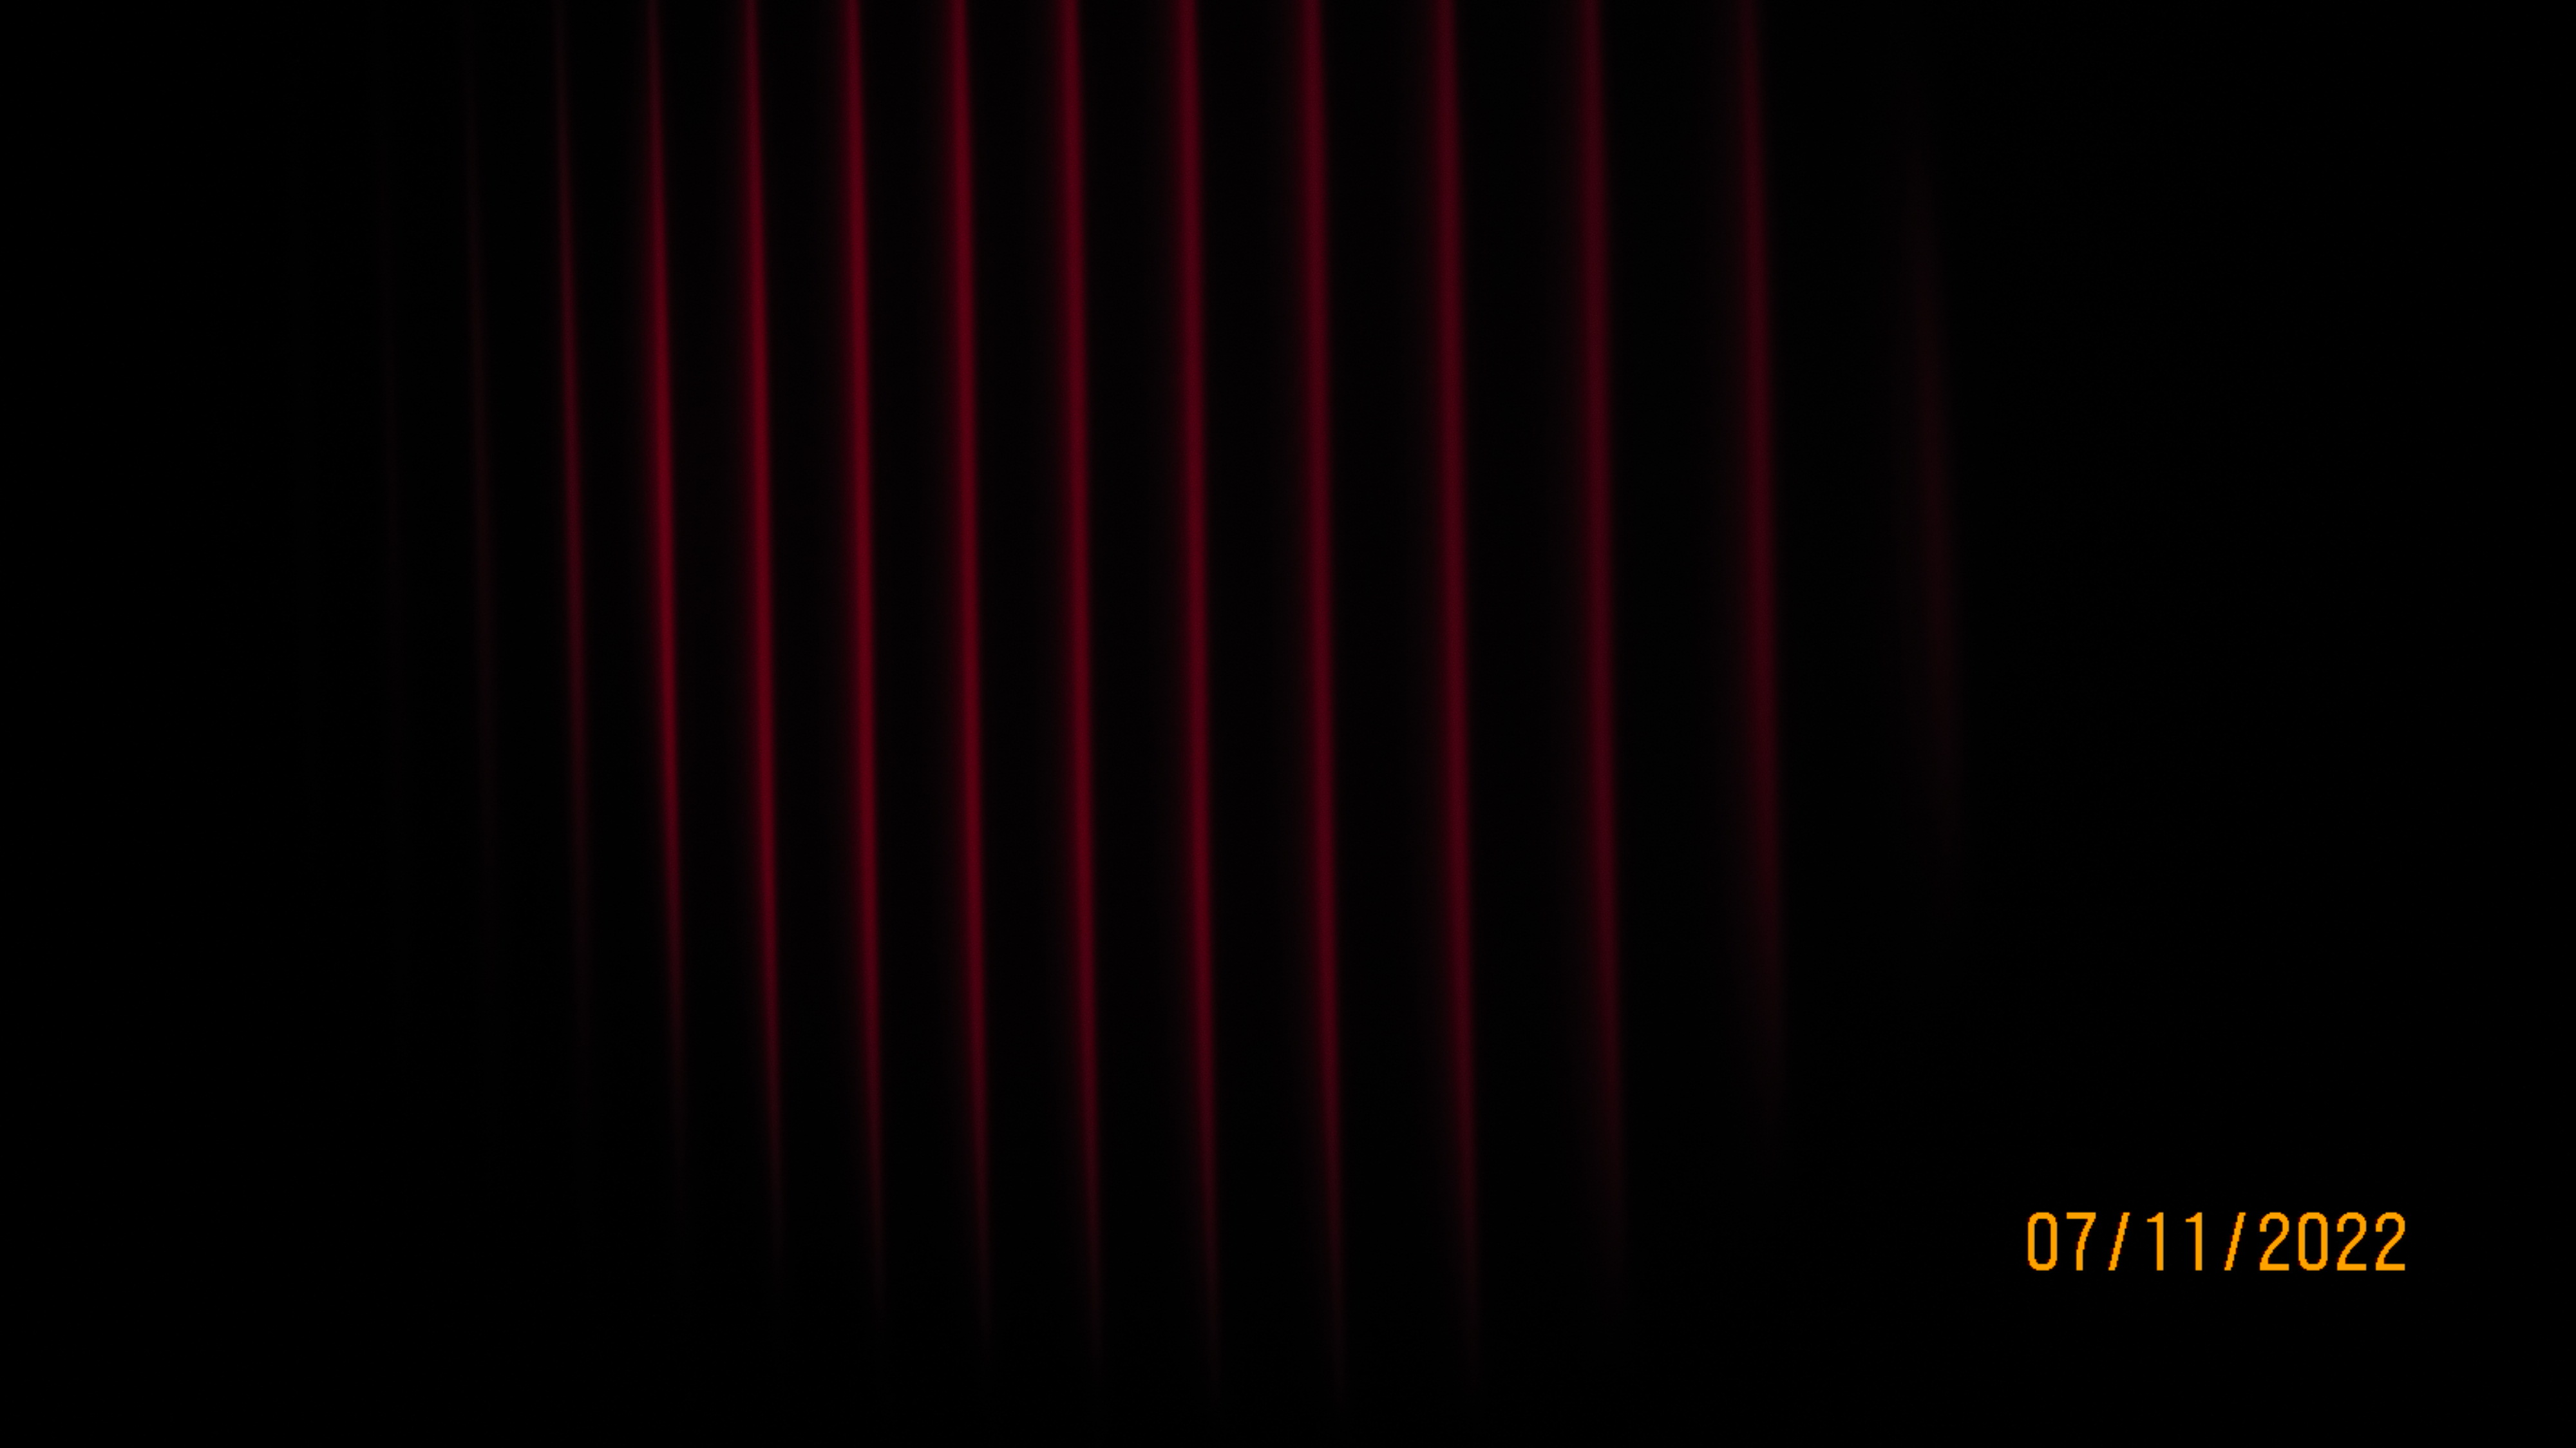
\includegraphics{../pictures/IMG_0005.JPG}%
      \caption{Für $B = \num{0}$.}%
      \label{fig:pic_rot_0}%
    \end{subfigure}%
    \hfill%
    \begin{subfigure}{0.48}%
      \centering%
      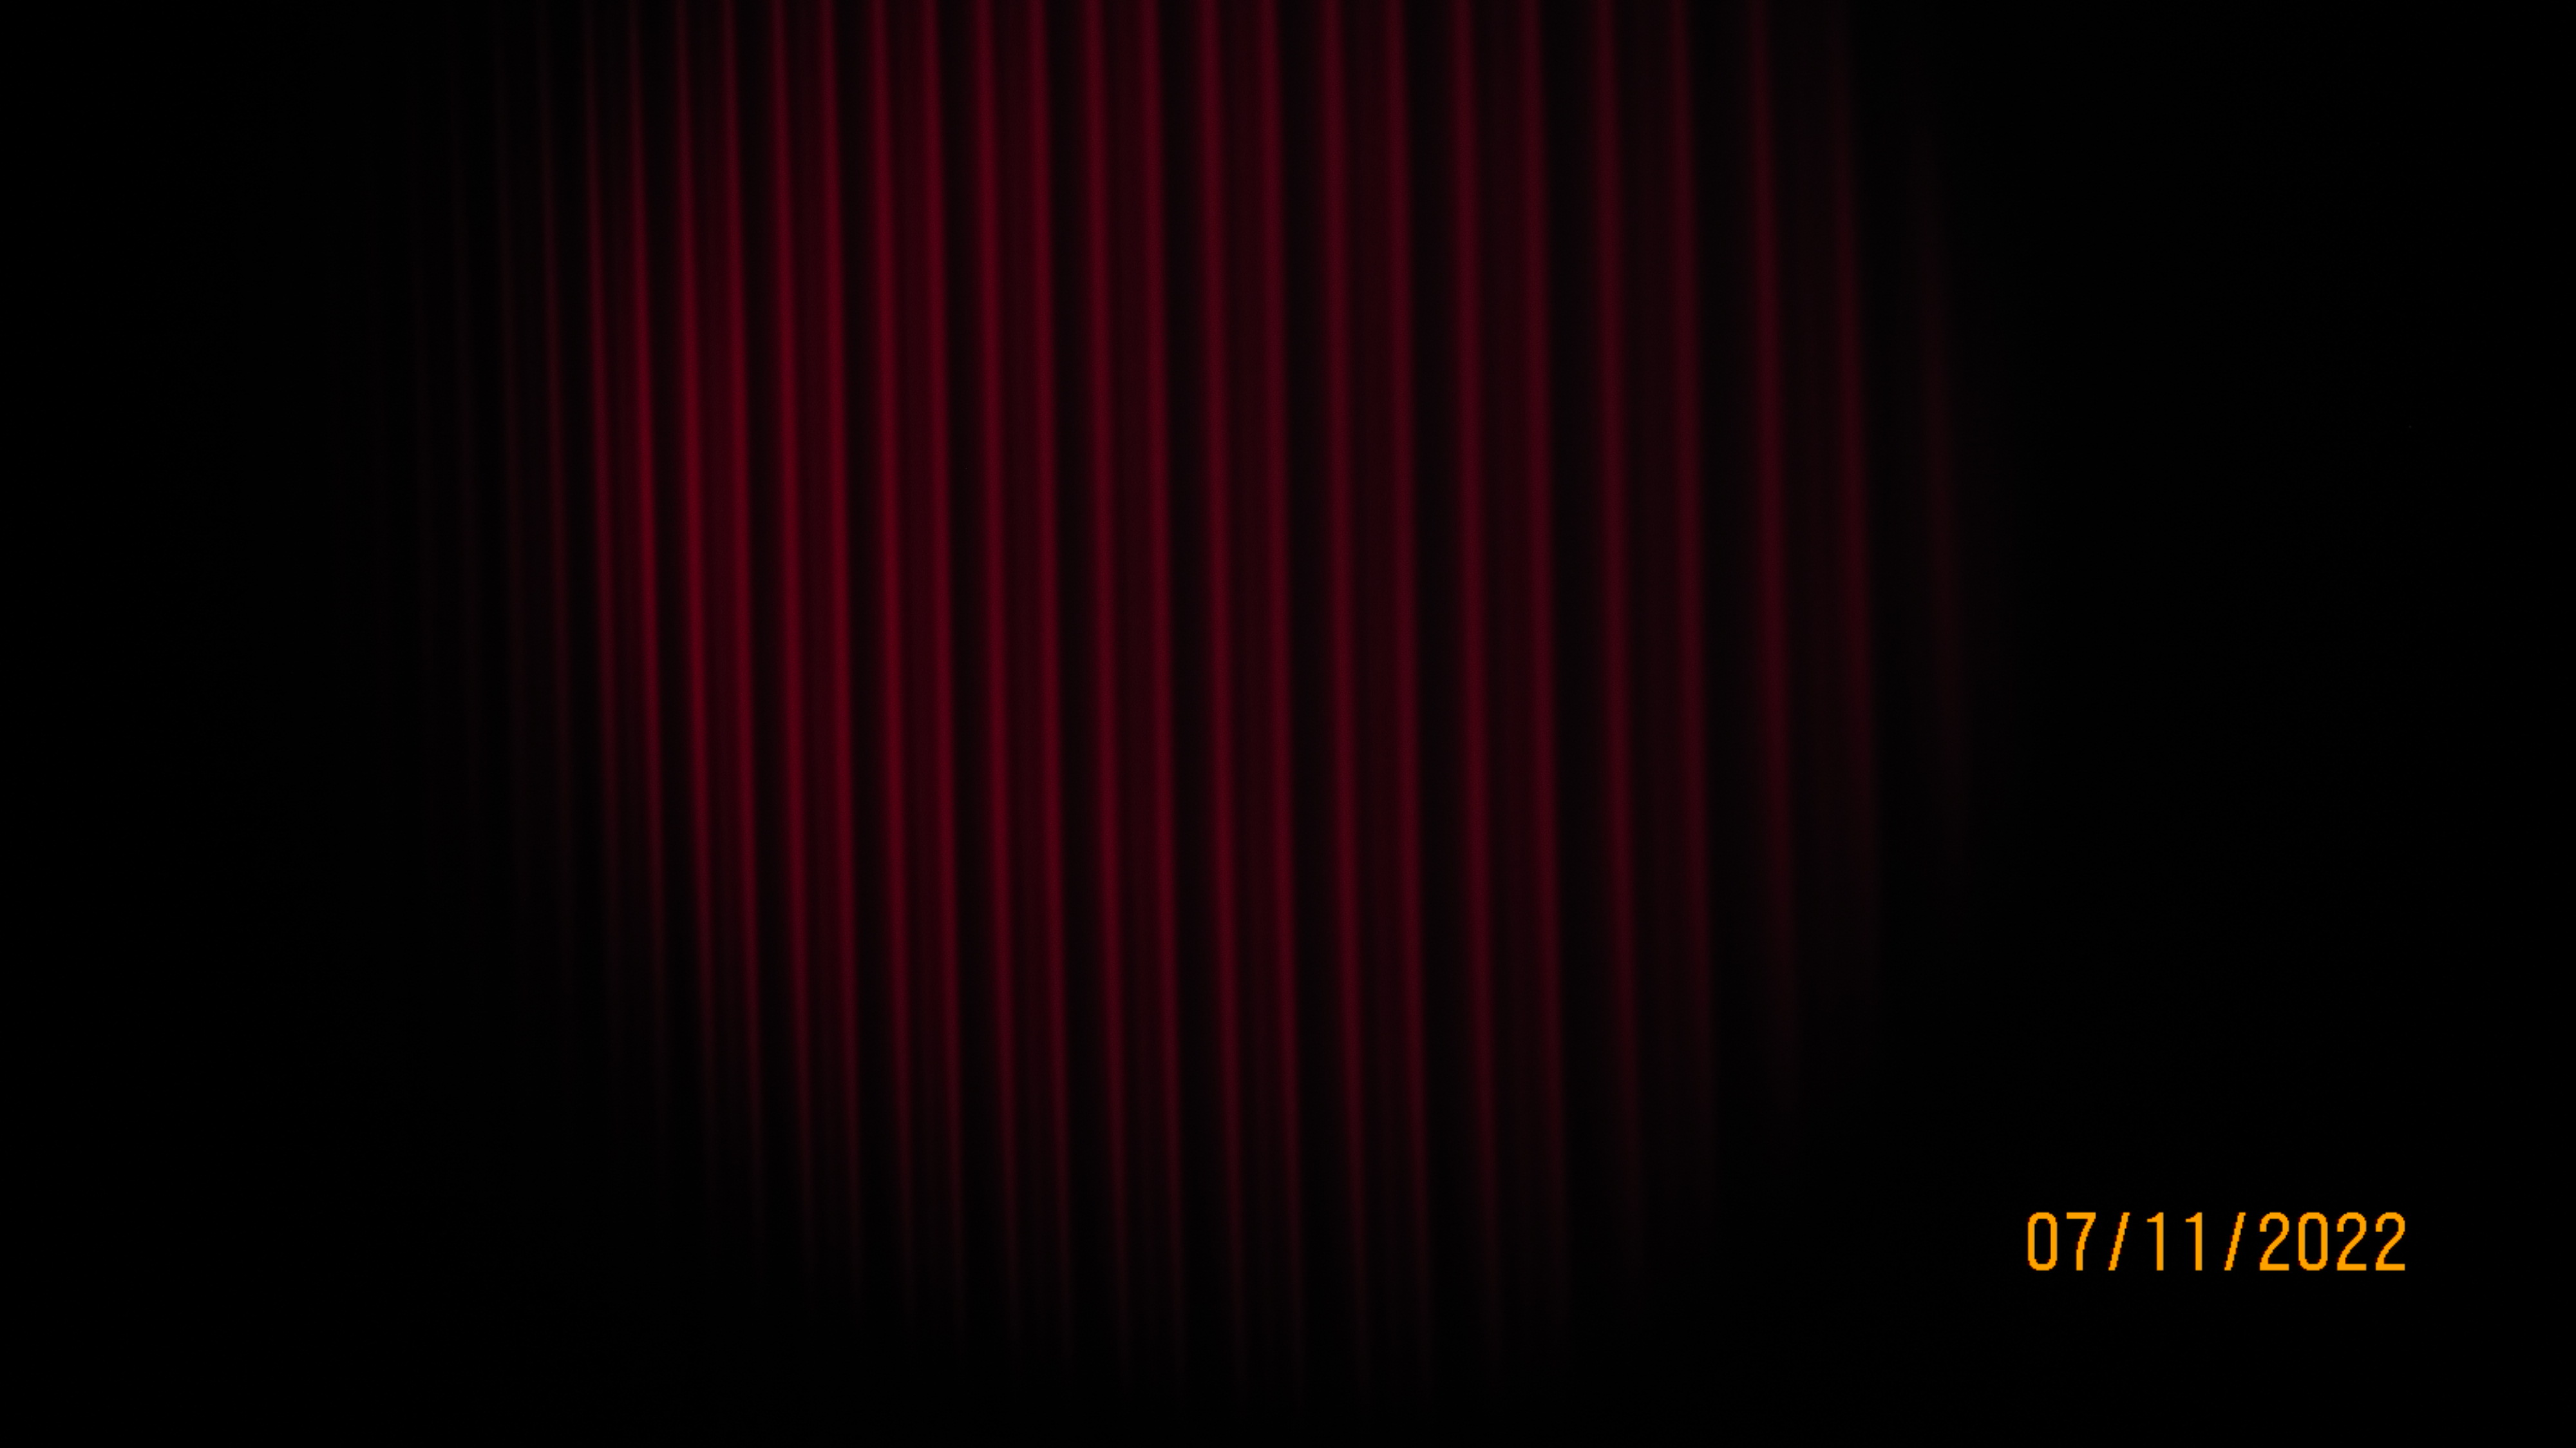
\includegraphics{../pictures/IMG_0006.JPG}%
      \caption{Für $B = \SI{583.49}{\milli\tesla}$.}%
      \label{fig:pic_rot_B}%
    \end{subfigure}%
    \caption{Die Aufnahmen der roten Spektrallinie mit und ohne Magnetfeld.}%
    \label{fig:rot}%
  \end{figure}

  \begin{table}
    \centering
    \caption{Die Abstände der Linien aus dem Fotos in \autoref{fig:rot} in Pixeln.}
    \label{tab:rotsigmas}
    \begin{tabular}{c S[table-format=3.0] S[table-format=3.0]}
      \toprule
      {Nr.} & {$\Delta s \mathbin{/} \text{px}$} & {$\delta s \mathbin{/} \text{px}$} \\
      \midrule
       1  &  136   &   56\\
       2  &  144   &   71\\
       3  &  153   &   80\\
       4  &  165   &   75\\
       5  &  167   &   85\\
       6  &  179   &   92\\
       7  &  190   &   93\\
       8  &  207   &   99\\
       9  &  218   &   111\\
      10  &  243     \\
      \bottomrule
    \end{tabular}
  \end{table}

  \noindent Zu den abgelesenen Werten werden jeweils $\SI{10}{px}$ als Messunsicherheit gewählt. Da sich die Abstände von links nach rechts vergrößern,
  wird die Formel \eqref{eqn:}
  \begin{equation*}
    \delta \lambda_i = \frac{1}{2} \frac{\delta s_i}{\Delta \tilde{s}_i} \Delta \lambda_\text{D}
  \end{equation*}
  angewendet, wobei 
  \begin{equation*}
    \Delta \tilde{s}_i = \frac{\Delta s_i + \Delta s_{i+1}}{2}\, .
  \end{equation*}
  Das Dispersionsgebiet $\Delta \lambda_\text{D}$ beträgt $\SI{489.13}{\nano\metre}$. 
  Anschließend wird aus den $\delta \lambda_i$ der Mittelwert berechnet, welcher sich zu 
  \begin{equation*}
    \delta \lambda = \SI{115(5)}{\nano\metre}
  \end{equation*}
  ergeben. 
  Mit dem Magnetfeld $B= \SI{583.49}{\milli\tesla}$, welches aus dem gemessenen Strom $I = \SI{}{\ampere}$ mit der Gleichung \eqref{eqn:bfield} berechnet wird, 
  ergibt sich für den Land\'{e}-Faktor nach \eqref{}
  \begin{equation*}
    g_{\text{rot}, \sigma} = \num{1.02(5)}\, .
  \end{equation*}

 
\subsection{Blaue Spektrallinie}

  \noindent 

  \subsubsection{$\sigma$-Linie}

    \noindent 

    \begin{figure}%
      \begin{subfigure}{0.48\textwidth}%
        \centering%
        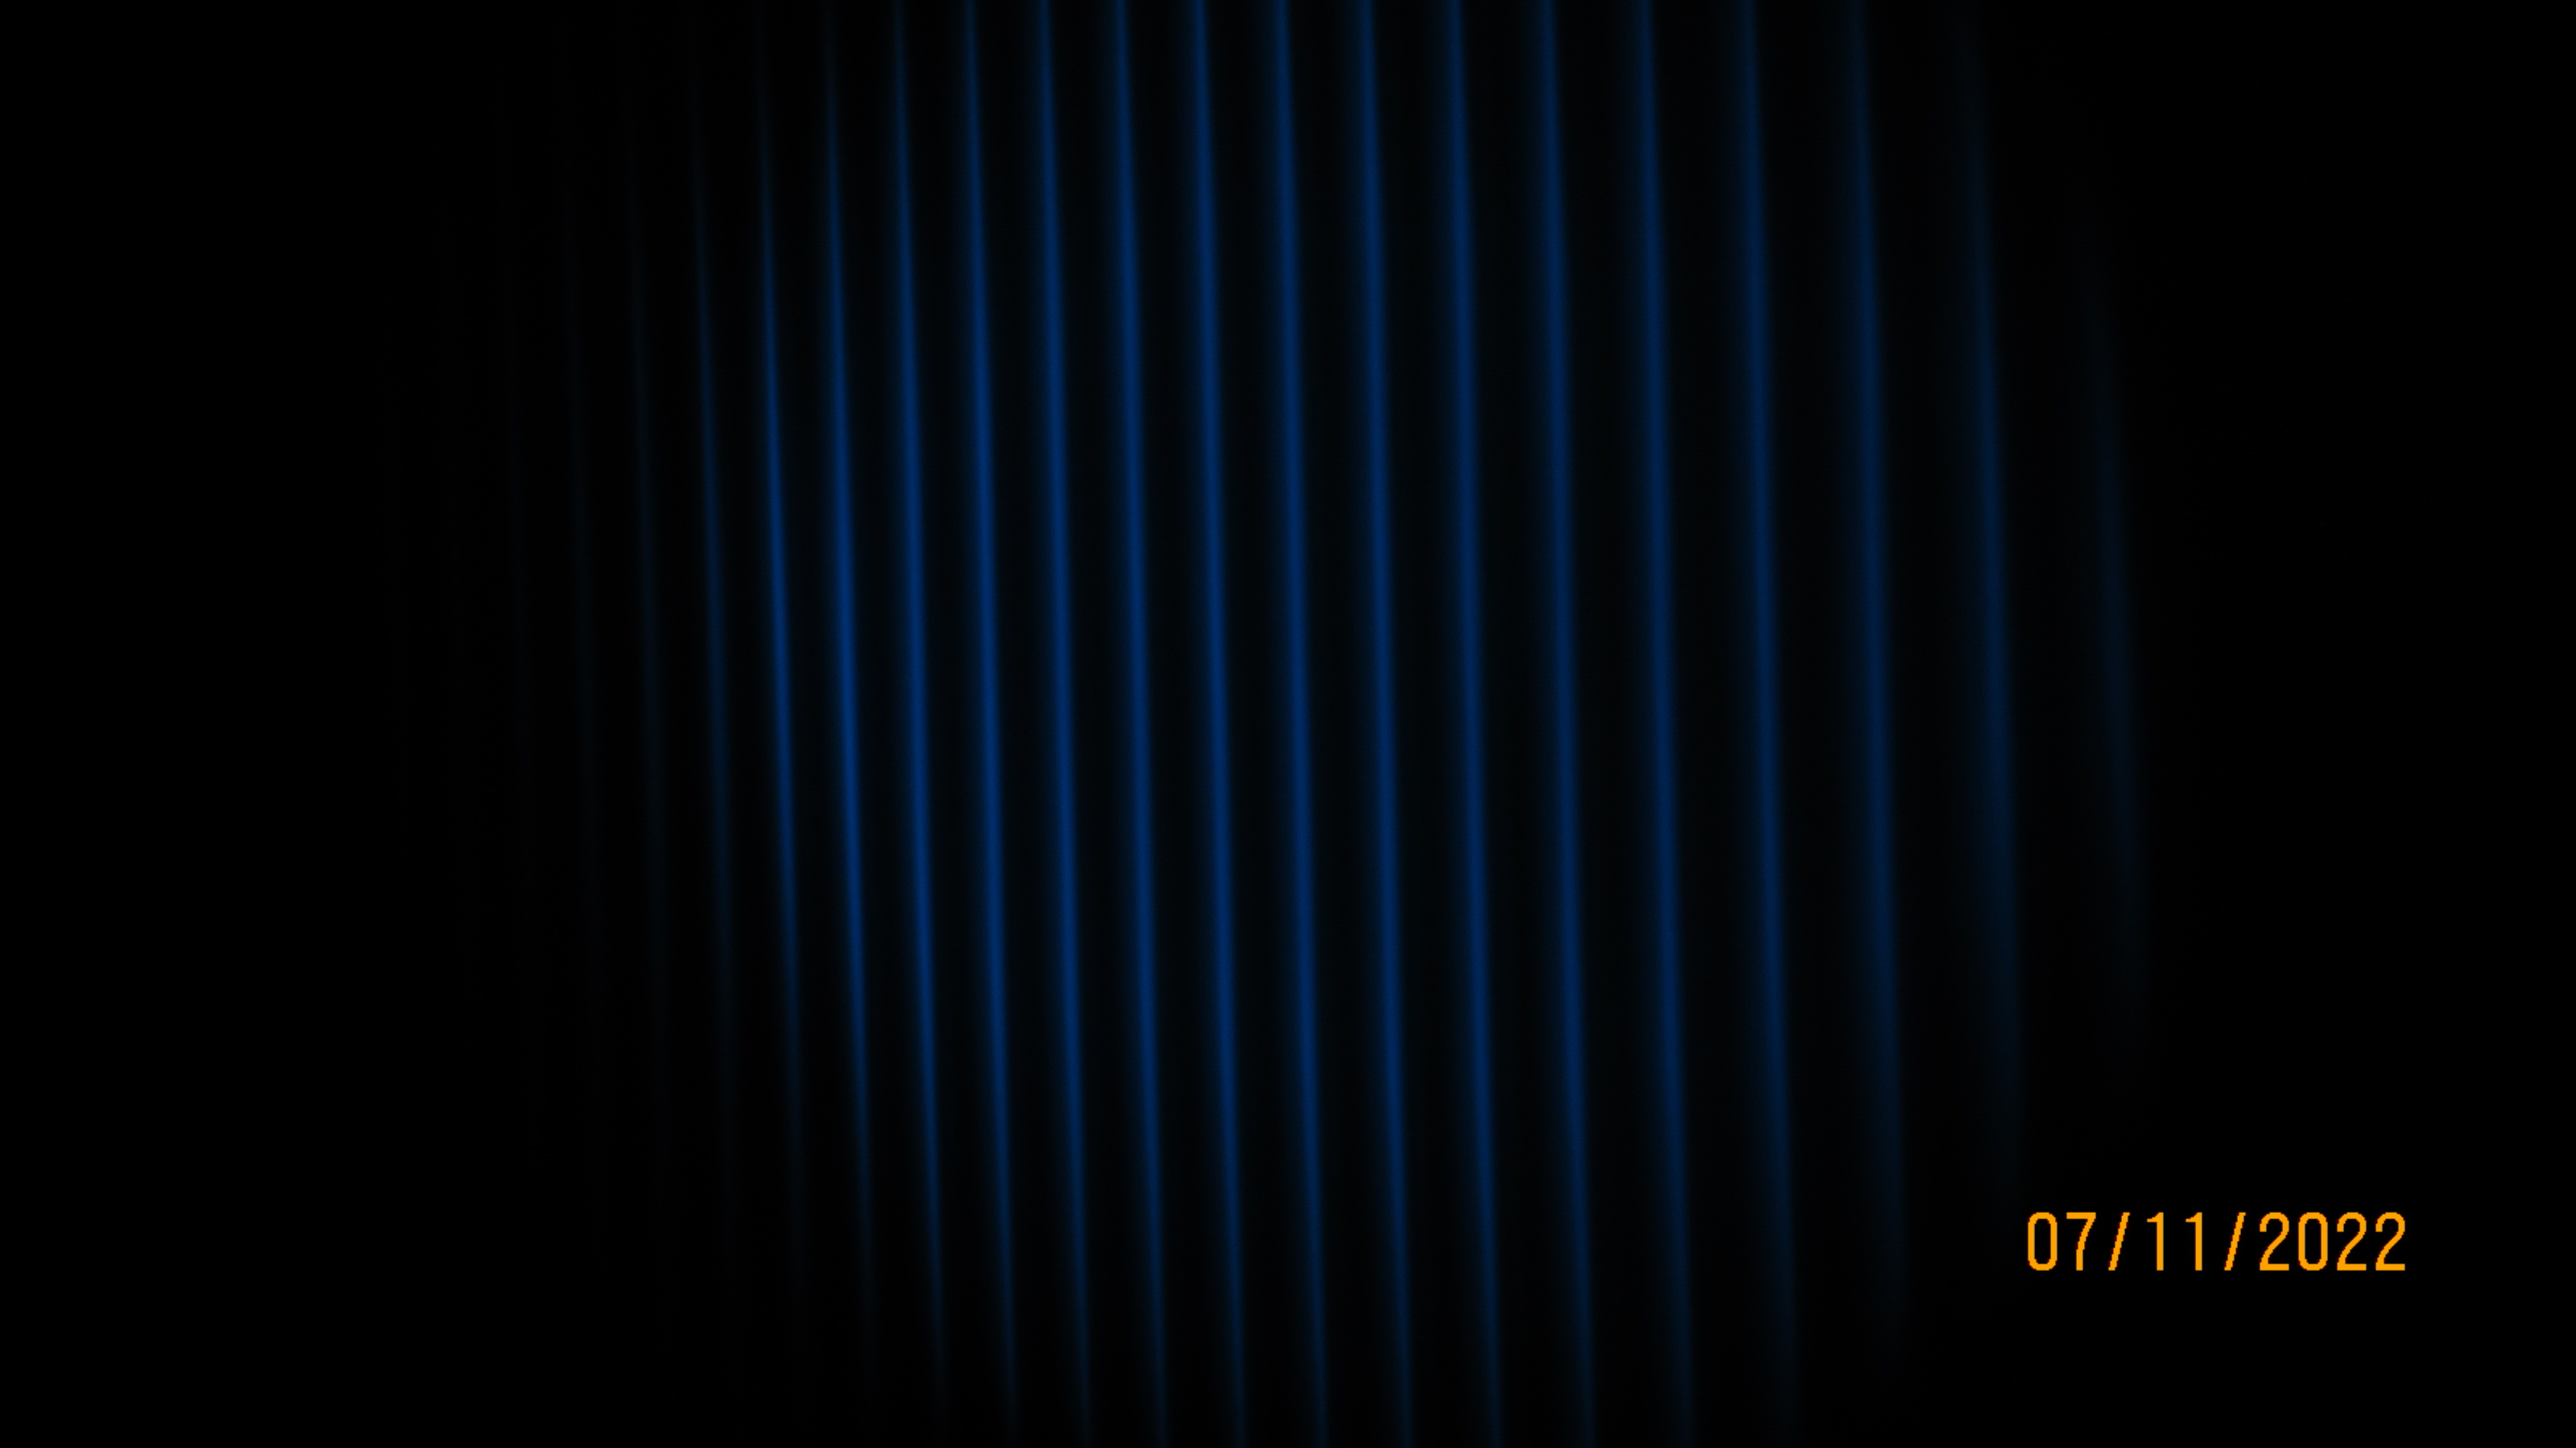
\includegraphics{../pictures/IMG_0007.JPG}%
        \caption{Für $B = \num{0}$.}%
        \label{fig:pic_blaus_0}%
      \end{subfigure}%
      \hfill%
      \begin{subfigure}{0.48}%
        \centering%
        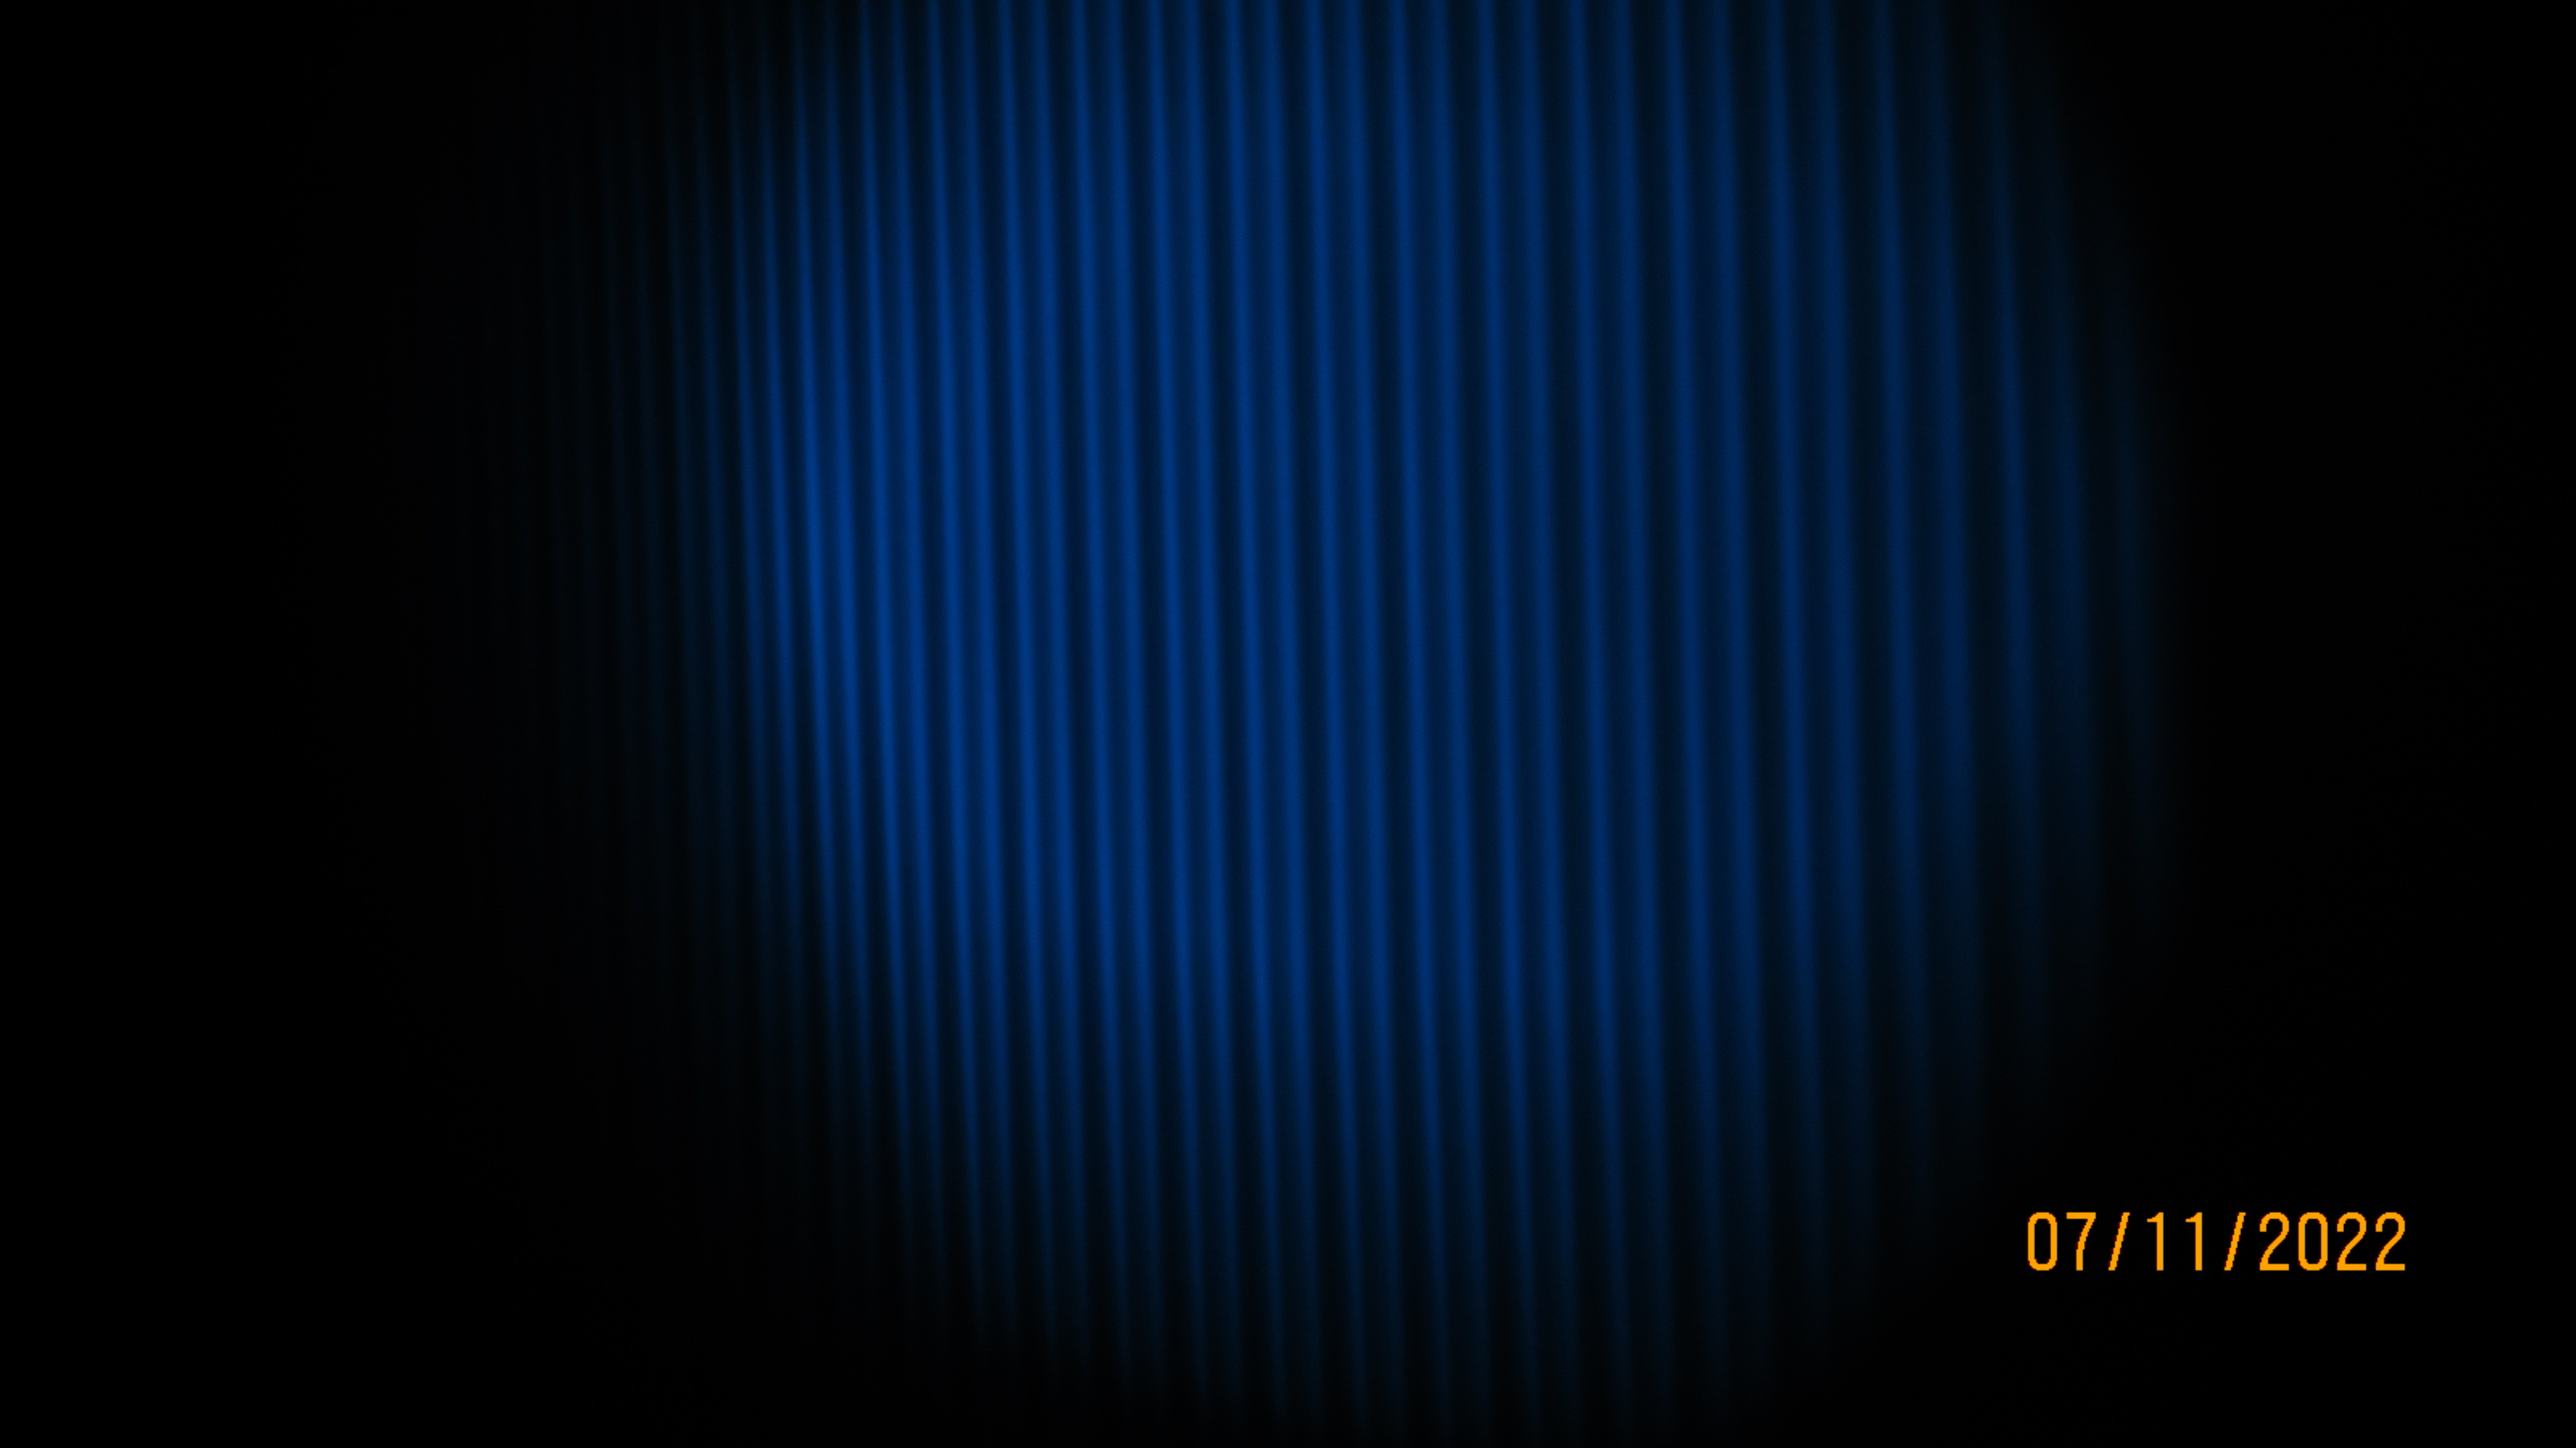
\includegraphics{../pictures/IMG_0008.JPG}%
        \caption{Für $B = \SI{330.99}{\milli\tesla}$.}%
        \label{fig:pic_blaus_B}%
      \end{subfigure}%
      \caption{Die Aufnahmen der blauen $\sigma$ Spektrallinie mit und ohne Magnetfeld.}%
      \label{fig:blaus}%
    \end{figure}

    \begin{table}
      \centering
      \caption{Die Abstände der Linien aus dem Fotos in \autoref{fig:blaus} in Pixeln.}
      \label{tab:blausigma}
      \begin{tabular}{c S[table-format=3.0] S[table-format=2.0]}
        \toprule
        {Nr.} & {$\Delta s \mathbin{/} \text{px}$} & {$\delta s \mathbin{/} \text{px}$} \\
        \midrule
         1  &  76   &   53\\
         2  &  95   &   53\\
         3  &  99   &   47\\
         4  &  105  &   50\\
         5  &  104  &   64\\
         6  &  109  &   61\\
         7  &  114  &   67\\
         8  &  117  &   60\\
         9  &  125  &   67\\
        10  &  128  &   63\\
        11  &  149  &   72\\
        12  &  145  &   60\\
        13  &  156  &   86\\
        14  &  165  &   68\\
        15  &  177  \\
        \bottomrule
      \end{tabular}
    \end{table}

  \subsubsection{$\pi$-Linie}

    \begin{figure}%
      \begin{subfigure}{0.48\textwidth}%
        \centering%
        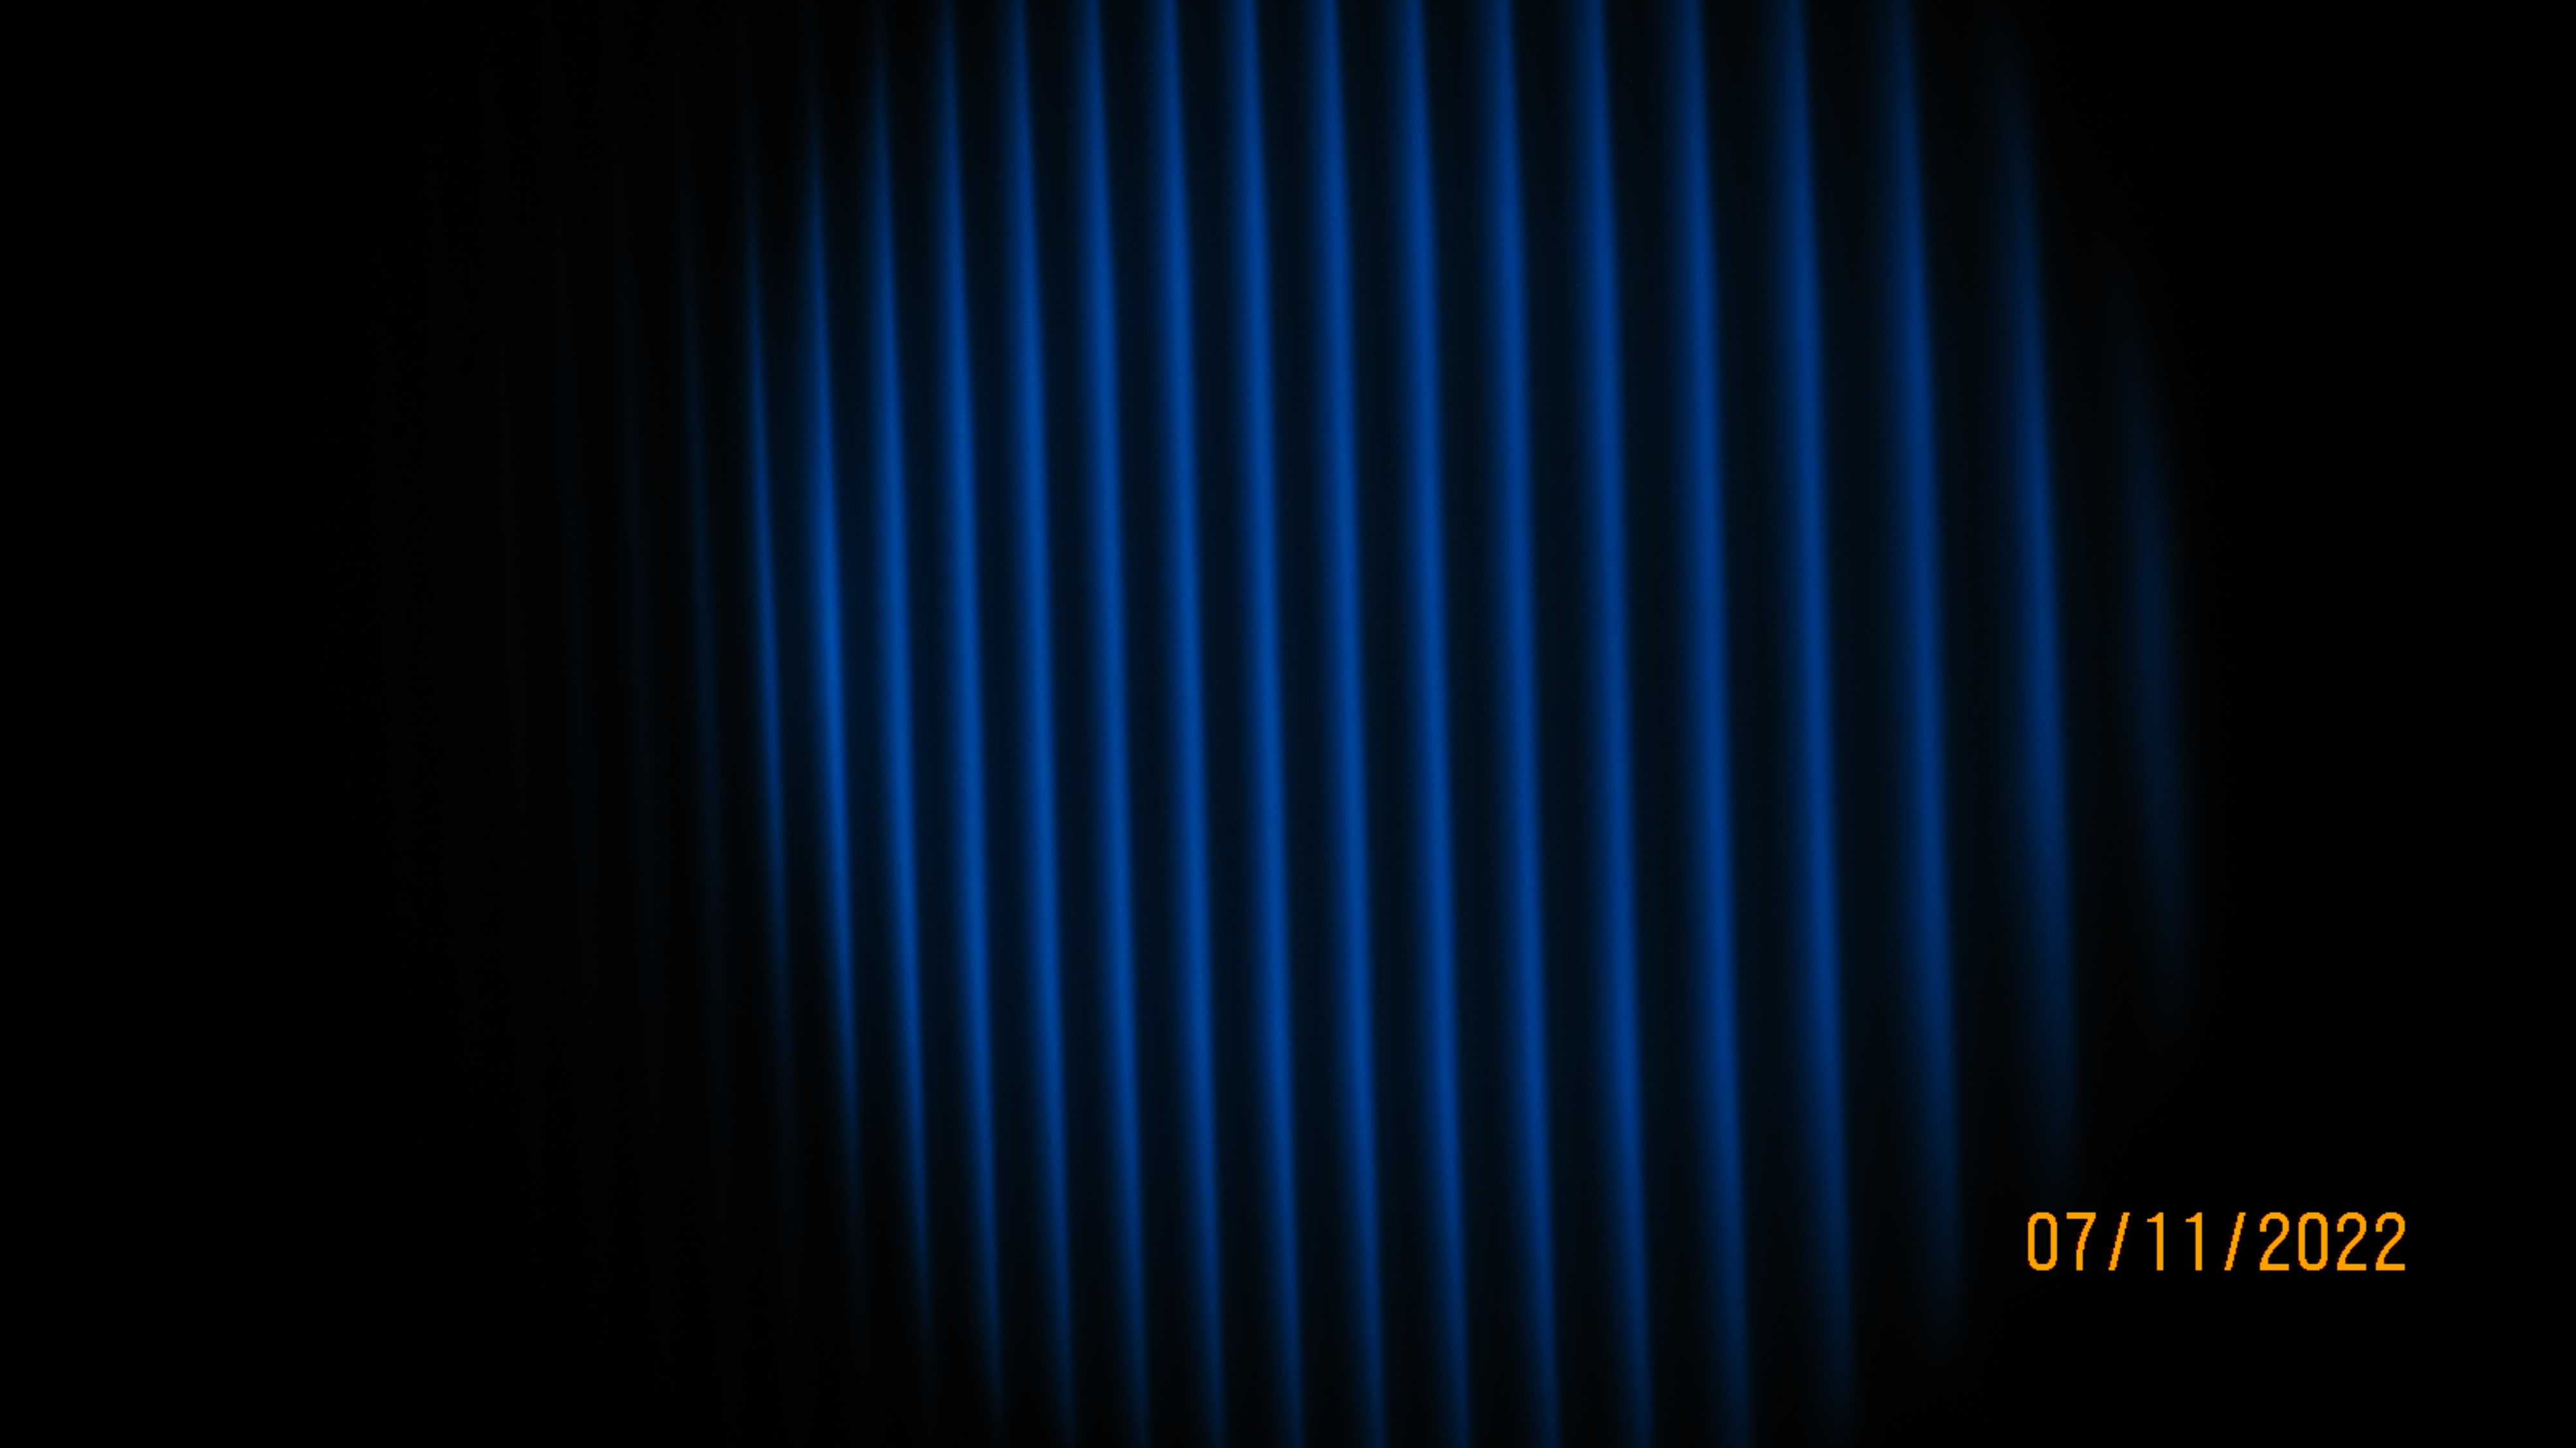
\includegraphics{../pictures/IMG_0009.JPG}%
        \caption{Für $B = \num{0}$.}%
        \label{fig:pic_blaup_0}%
      \end{subfigure}%
      \hfill%
      \begin{subfigure}{0.48}%
        \centering%
        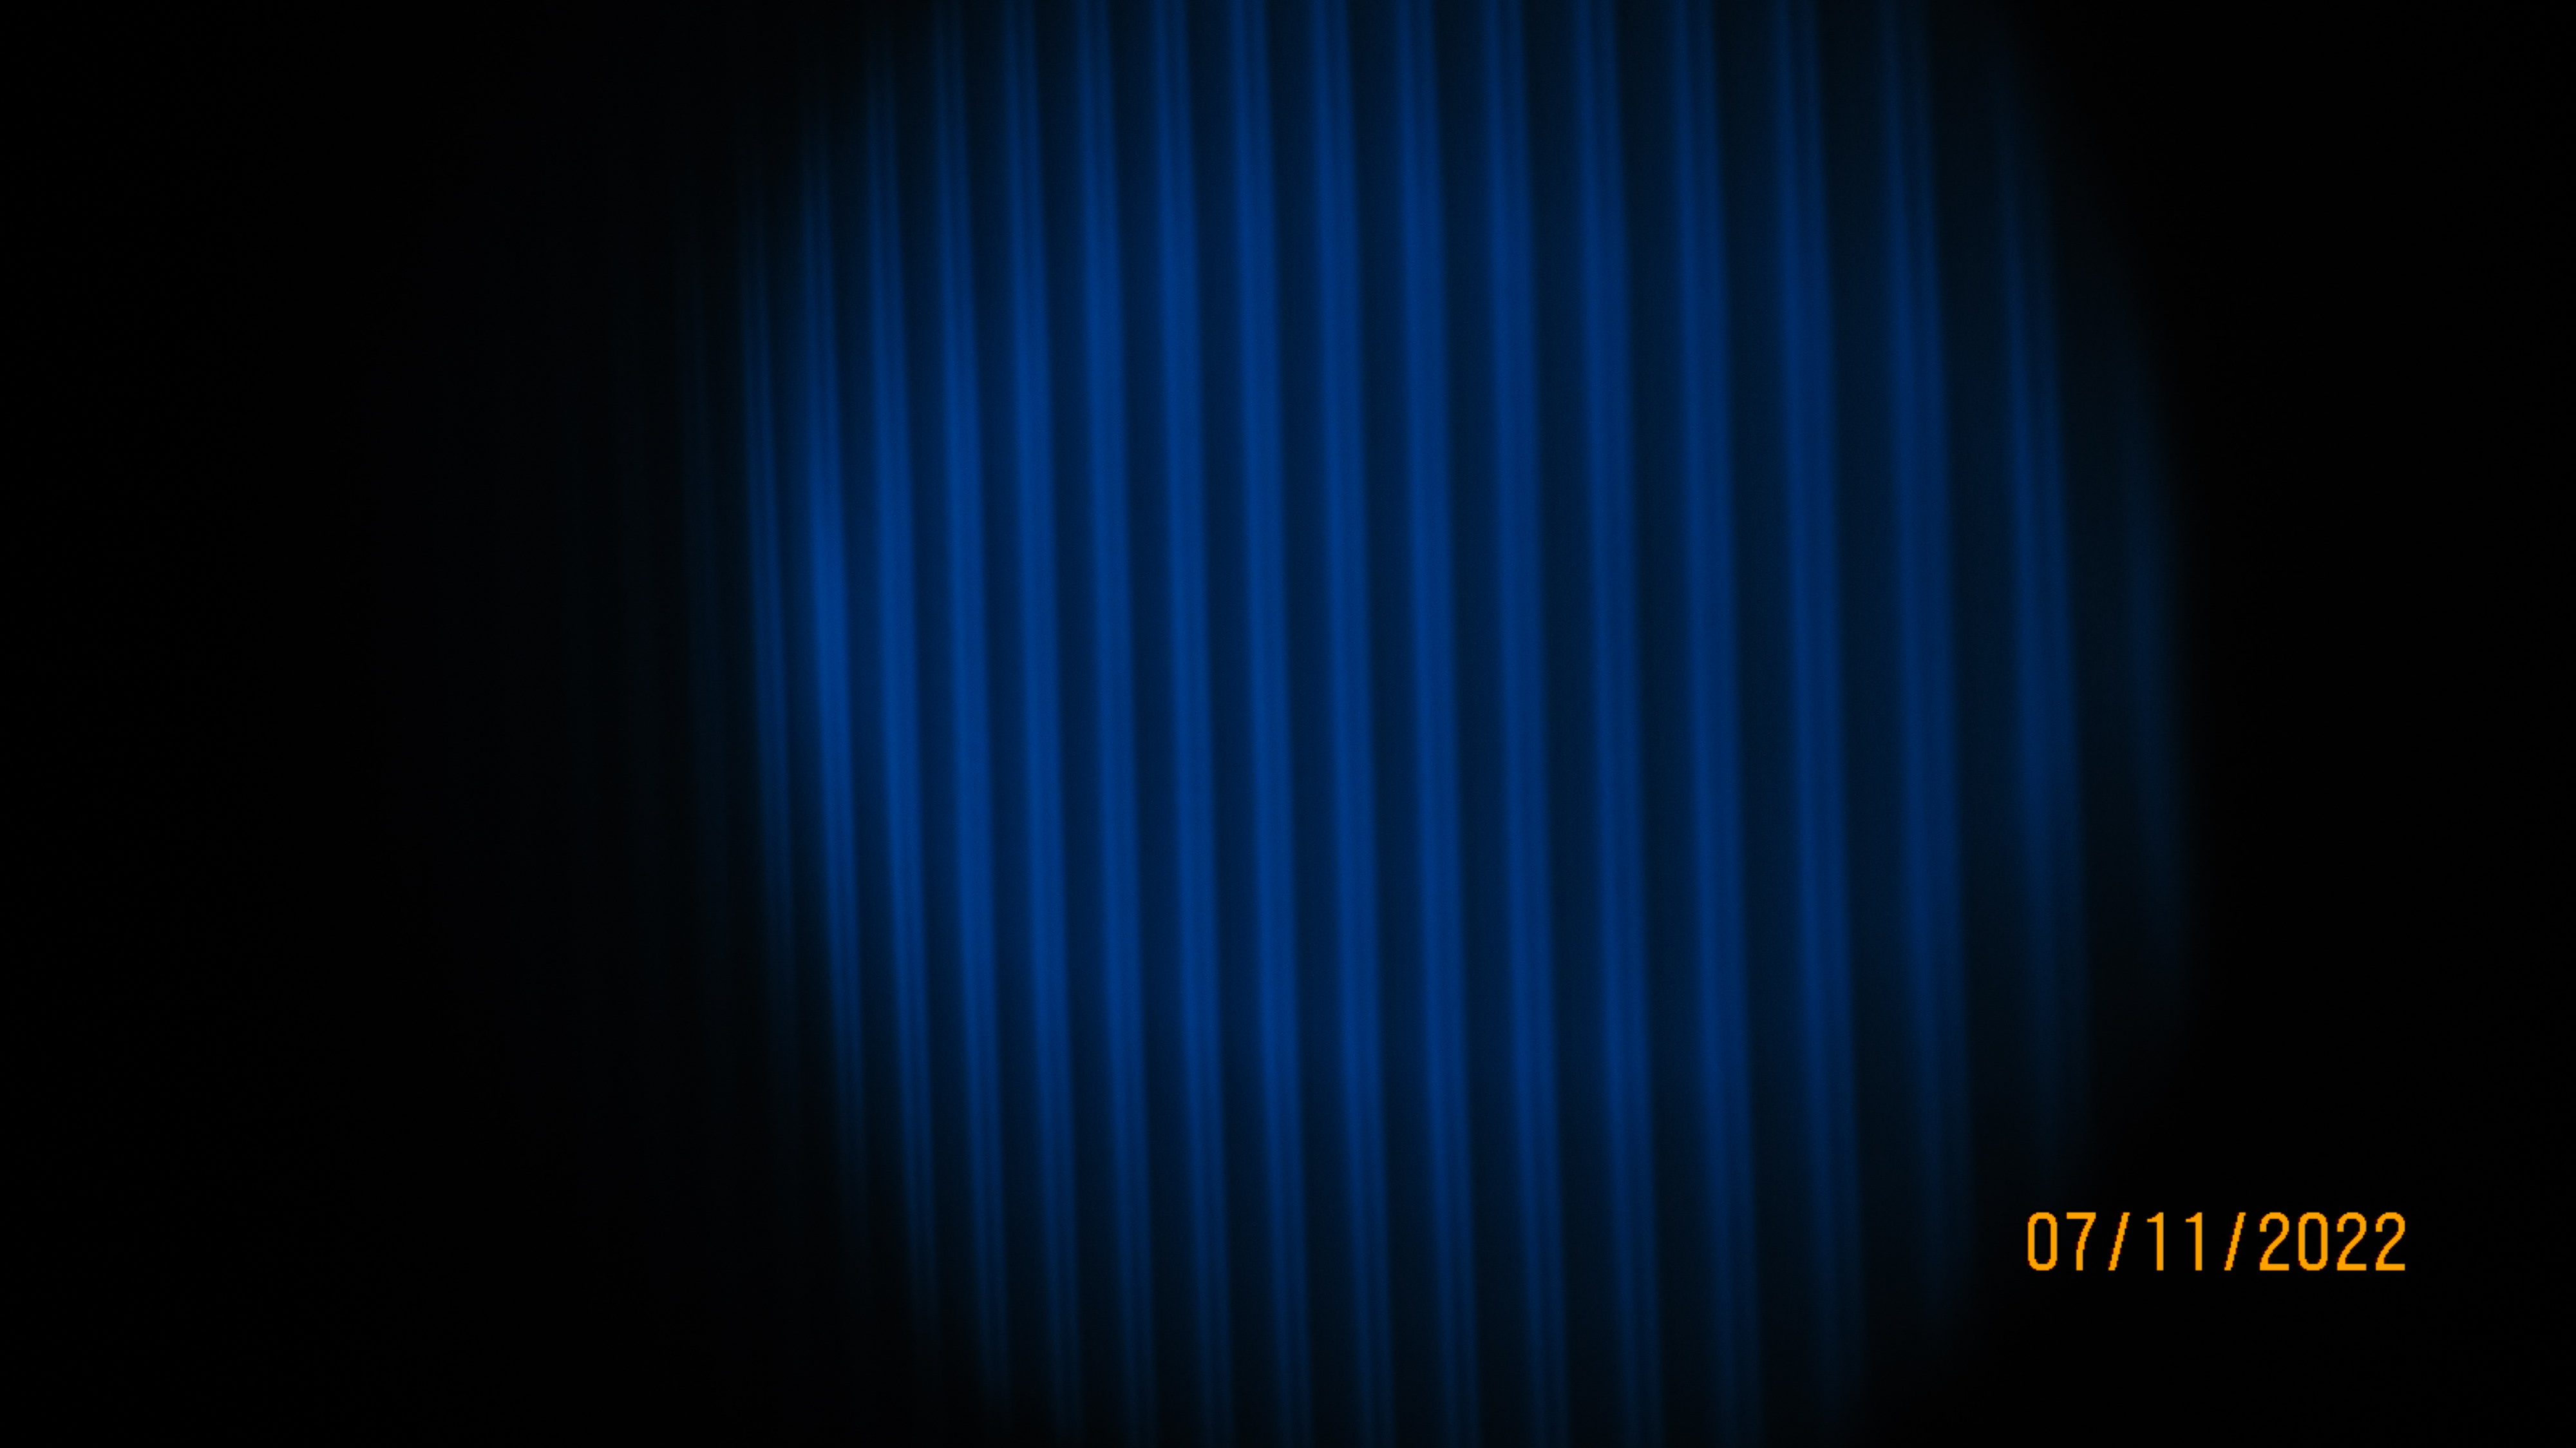
\includegraphics{../pictures/IMG_0010.JPG}%
        \caption{Für $B = \SI{583.50(7143)}{\milli\tesla}$.}%
        \label{fig:pic_blaup_B}%
      \end{subfigure}%
      \caption{Die Aufnahmen der blauen $\pi$ Spektrallinie mit und ohne Magnetfeld.}%
      \label{fig:blaup}%
    \end{figure}

    \begin{table}
      \centering
      \caption{Die Abstände der blauen $\pi$ Linien aus dem Fotos in \autoref{fig:blaup} in Pixeln.}
      \label{tab:blaupi}
      \begin{tabular}{c S[table-format=3.0] S[table-format=2.0]}
        \toprule
        {Nr.} & {$\Delta s \mathbin{/} \text{px}$} & {$\delta s \mathbin{/} \text{px}$} \\
        \midrule
         1  & 99    &  17 \\ 
         2  & 101   &  26 \\ 
         3  & 107   &  27 \\ 
         4  & 106   &  23 \\ 
         5  & 110   &  31 \\ 
         6  & 113   &  23 \\ 
         7  & 119   &  25 \\ 
         8  & 127   &  28 \\ 
         9  & 129   &  31 \\ 
        10  & 136   &  42 \\ 
        11  & 136   &  38 \\ 
        12  & 154   &  38 \\ 
        13  & 157   &  47 \\ 
        14  & 172   &  52 \\ 
        15  & 180  &   \\
        \bottomrule
      \end{tabular}
    \end{table}